\documentclass[ai,article,submit,pdftex,moreauthors]{Definitions/mdpi} 

%=================================================================
\firstpage{1} 
\makeatletter 
\setcounter{page}{\@firstpage} 
\makeatother
\pubvolume{1}
\issuenum{1}
\articlenumber{0}
\pubyear{2025}
\copyrightyear{2025}
\datereceived{ } 
\daterevised{ } 
\dateaccepted{ } 
\datepublished{ } 
\hreflink{https://doi.org/} 

%=================================================================
\usepackage{algorithm} % Provides the algorithm floating environment
\usepackage{algpseudocode} % Provides the algorithmic environment for writing pseudocode
\usepackage{siunitx} % For proper unit formatting
\usetikzlibrary{positioning}
\usepackage{booktabs} % For professional table formatting
\usepackage{bbm} % For rendering blackboard bold characters

%=================================================================
% Add packages and commands here.
% The following packages are loaded in our class file: fontenc, inputenc, calc, indentfirst, fancyhdr, graphicx, epstopdf, lastpage, ifthen, float, amsmath, amssymb, lineno, setspace, enumitem, mathpazo, booktabs, titlesec, etoolbox, tabto, xcolor, colortbl, soul, multirow, microtype, tikz, totcount, changepage, upgreek, array, tabularx, pbox, ragged2e
%=================================================================
%% Please use the following mathematics environments:
%% Theorem, Lemma, Corollary, Proposition, Characterization, Property, Problem, Example, ExamplesandDefinitions, Hypothesis, Remark, Definition
%% For proofs, please use the proof environment (the amsthm package is loaded by the MDPI class).

%=================================================================

%--------------------
% Title
%--------------------
\Title{Explainable Fake News Detection with Large Language Models via Mental-Model Approximation}

% MDPI internal command: Title for citation in the left column
\TitleCitation{Explainable Fake News Detection with Large Language Models via Mental-Model Approximation}

% Author Orchid ID: enter ID or remove command
\newcommand{\orcidauthorA}{0000-0003-3609-112X} % Pavlo Radiuk
\newcommand{\orcidauthorB}{0000-0003-0739-9678} % Oleksander Barmak
\newcommand{\orcidauthorC}{0000-0002-8043-0785} % Iurii Krak

% Authors, for the paper (add full first names)
\Author{Pavlo Radiuk $^{1}$\orcidA{}, Oleksander Barmak $^{1}$\orcidB{} and Iurii Krak $^{2,3}$\orcidC{}}

% MDPI internal command: Authors, for metadata in PDF
\AuthorNames{Pavlo Radiuk, Oleksander Barmak, Pavlo Radiuk, Iurii Krak}

% MDPI internal command: Authors, for citation in the left column
\isAPAStyle{%
       \AuthorCitation{Radiuk, P., Barmak, O., \& Krak, I.}
         }{%
        \isChicagoStyle{%
        \AuthorCitation{Radiuk, Pavlo, Oleksander Barmak, and Iurii Krak.}
        }{
        \AuthorCitation{Radiuk, P.; Barmak, O.; Krak, I.}
        }
}

% Affiliations / Addresses (Add after \address if there is only one affiliation.)
\address{%
$^{1}$ \quad Department of Computer Science, Khmelnytskyi National University, 11 Instytuts’ka Str., 29016 Khmelnytskyi, Ukraine; ostrovskyiz@khmnu.edu.ua (Z.O.); barmako@khmnu.edu.ua (O.B.)\\
$^{2}$ \quad Department of Theoretical Cybernetics, Taras Shevchenko National University of Kyiv, 
4d Akademika Glushkova Ave, 03680 Kyiv, Ukraine; iurii.krak@knu.ua (I.K.)\\
$^{3}$ \quad Laboratory of Communicative Information Technologies, V.M. Glushkov Institute of Cybernetics, 
40 Akademika Glushkova Ave, 03187 Kyiv, Ukraine}

% Contact information of the corresponding author
\corres{Correspondence: radiukp@khmnu.edu.ua; Tel.: +380-97-854-9146}

% Abstract
\abstract{High-performing large language models (LLMs) excel at misinformation detection but typically act as black boxes, limiting accountability in safety-critical use. In this work, we propose a transparent two-stage pipeline that approximates LLM decisions with an interpretable mental model built from domain-grounded features. Stage~1 elicits characteristic features of misinformation using prompt-engineered LLM guidance and deterministic NLP, with explicit mechanisms that compute numeric values in [0,1] and record evidence (token spans, quotes, links). Stage~2 trains a lightweight classifier on these features to approximate LLM outputs and produces a structured expert report that links each decision to verifiable evidence. We formalize the pipeline via four mappings (text, characteristic features, numeric features, ML model, explanation), define feature metrics (paraphrasing, subjectivity, header--summary coherence, unusual or manipulative language, sentiment and narrative consistency, fact confirmation, selective quoting), and prescribe a rigorous evaluation protocol: stratified splits, PCA/MDS/t-SNE visualization, accuracy/precision/recall/F1/AUC, and leakage controls. Using ISOT and LIAR, the approach is designed to match deep baselines while substantially improving traceability and auditability.}

% Keywords
\keyword{fake news detection; explainable AI; large language models; mental-model approximation; feature mechanisms; human-in-the-loop; support vector machine}

%%%%%%%%%%%%%%%%%%%%%%%%%%%%%%%%%%%%%%%%%%
\begin{document}

%%%%%%%%%%%%%%%%%%%%%%%%%%%%%%%%%%%%%%%%%%
\section{Introduction}

\subsection{Motivation and Contributions}
Deep models, including LLMs, achieve strong performance in misinformation detection but often operate as black boxes. This reduces trust and impedes responsible deployment. We address this by approximating LLM decisions within a compact, interpretable mental model constructed from characteristic features of misinformation derived from LLM- and NLP-guided analysis. The proposed pipeline scales prior authors' work on transition-based explainability to news content and emphasizes transparent evidence trails that can be audited by domain experts.

The goal of this study is to improve the fidelity and transparency of fake news detection by approximating LLM decisions with a compact, interpretable mental model composed of domain-grounded features and an open ML classifier.

\noindent\textit{Major contributions:}
(1) A formal, four-mapping framework that transforms text into explanations via characteristic features and a learned ML proxy, with explicit metadata to support traceable, expert-facing reports.
(2) A feature-mechanism library that couples prompt-engineered LLM guidance with deterministic NLP code, yielding numeric features in $[0,1]$ and the text spans that contributed to them; this supports post-processing such as annotation of subjective tokens and selective quoting analysis.
(3) A rigorous evaluation protocol---including dimensionality-reduction validation, stratified train--test splits, standard metrics (accuracy, precision, recall, F1, AUC), and out-of-distribution checks---that enables fair comparison against reported baselines while avoiding leakage.

\subsection{State of the Art}
Classical ML pipelines with TF--IDF or lexicon-based features (e.g., Na\"{i}ve Bayes, SVM) achieve strong in-domain performance but are brittle to distribution shifts and dynamic language \cite{amer2021context,ahmed2022development}. Deep pretraining (e.g., BERT) improved contextual understanding and accuracy \cite{devlin2018bert,keya2021augfakebert}; hybrid CNN--BERT models (FakeBERT) report up to $98.90\%$ accuracy \cite{kaliyar2021fakebert}, and dual-input variants process headlines and bodies in parallel \cite{farokhian2022parallel}. Recent works consider robustness to LLM style attacks, bias in detectors, and knowledge-augmented LVLMs \cite{wu2023sheep,park2024adstyle,su2023biased,liu2024fkaowl}.

\subsection{Previous Works}
Our work scales a previously validated, transition-matrix explainability program from the same research line to the LLM setting, preserving interpretability while approximating high-capacity decisions with user-friendly features \cite{radiuk2024matrices,barmak2024healthcare}.

Surveys synthesize theories and detection methods across social, content, and knowledge signals \cite{zhou2020survey,tandoc2019facts,pennycook2021psychology}. Traditional pipelines combine TF--IDF, sentiment, and imputation strategies, achieving high reported in-domain accuracy (e.g., $99.8\%$) but raising concerns about generalization and leakage \cite{amer2021context,ahmed2022development,villela2023review}. BERT-based and hybrid deep approaches (FakeBERT; parallel BERT) substantially improve accuracy and representation power \cite{kaliyar2021fakebert,farokhian2022parallel}, while recent studies stress robustness and bias considerations in the LLM era \cite{wu2023sheep,park2024adstyle,su2023biased,leite2023weak}.

\subsection{Purposes and Objectives of the Study}
We target reliable, explainable detection of fake news that retains LLM-level competence while being auditable. Specifically, we: (i) define an interpretable feature space for misinformation; (ii) design feature mechanisms that map text to $[0,1]$-valued features and evidence; (iii) train a simple, transparent ML model on feature vectors to approximate LLM decisions; and (iv) produce structured expert reports linking features to text spans. These objectives guide the method and evaluation.

Our objective is to construct a proxy model that is: (i) faithful enough to approximate LLM judgments; (ii) transparent enough for expert scrutiny; and (iii) robust to dataset shifts via explicit feature definitions and human-in-the-loop validation. The tasks are: define characteristic features; instantiate feature mechanisms (LLM-guided prompts and deterministic NLP); learn a lightweight classifier; and design an expert-report template with verifiable evidence.

%%%%%%%%%%%%%%%%%%%%%%%%%%%%%%%%%%%%%%%%%%
\section{Methods}\label{sec:methods}

\subsection{Proposed Approach}\label{subsec:approach}
We explain the decisions of LLMs by approximating them with decisions of simple, interpretable machine-learning (ML) models whose features have clear semantics and evidence traces. The core idea is to relate a high-dimensional LLM embedding space to a low-dimensional, expert-defined feature space via a data-driven linear transition, and then to use that transition at inference time to produce feature-level explanations for the LLM's outputs. The proposed pipeline remains two-phased: a \emph{Design Stage} that learns the mapping between spaces, and a \emph{Detection \& Explanation Stage} that deploys this mapping with an auditable report.

\paragraph{Design Stage.}
Given a labeled training corpus, we compute two representations for the same set of $m$ texts:
\begin{equation}\label{eq:Adef}
A \in \mathbb{R}^{m \times k} \quad \text{(LLM embeddings)},
\end{equation}
\begin{equation}\label{eq:Bdef}
B \in \mathbb{R}^{m \times \ell} \quad \text{(interpretable feature vectors)}.
\end{equation}

The rows of $A$ are document-level embeddings obtained from a chosen LLM embedding procedure (Section~\ref{subsec:embeddings}). The rows of $B$ are numeric vectors composed of expert-understandable features derived from text (Section~\ref{subsec:mlfeatures}). We learn a linear transition matrix $T \in \mathbb{R}^{k \times \ell}$ that maps the LLM space to the mental-model feature space in the least-squares sense:
\begin{equation}\label{eq:ls}
\min_{T}\;\|AT - B\|_F^2,
\end{equation}
with the standard Moore--Penrose pseudoinverse solution
\begin{equation}\label{eq:T}
T = A^{+} B,
\end{equation}
where $A^{+}$ is computed via SVD with a numerically stable tolerance.

During this stage we validate $A$, $B$, and $AT$ using dimensionality reduction (PCA/MDS/t-SNE) and quantitative quality indicators (e.g., explained variance or stress).

\paragraph{Detection and Explanation Stage.}
For a new text $x$ we compute its LLM embedding $a^{\ast}\!\in\!\mathbb{R}^{1\times k}$, then project it into the interpretable feature space:
\begin{equation}\label{eq:proj}
b^{\ast} = a^{\ast} T \in \mathbb{R}^{1\times \ell}.
\end{equation}

We then (i) score $b^{\ast}$ with a lightweight classifier (linear SVM or logistic regression trained on $B$), and (ii) generate an explanation by reporting the feature values and surfacing feature-specific evidence (token spans, quotes, links). This yields a decision accompanied by explicit, verifiable reasons.

\subsection{Requirements and Characteristics of the Training Dataset}\label{subsec:data}
The dataset must allow construction of both $A$ and $B$ for identical items and support reliable evaluation of~\eqref{eq:ls}--\eqref{eq:proj}. We consider three complementary acquisition paths (usable alone or in combination).

\paragraph{Curated public corpora.}
Use annotated news corpora whose items match the task (article-level records with titles, leads, bodies; clear labels such as \texttt{fake}/\texttt{real} or multi-class veracity). Requirements include: topical diversity; expert or reputable fact-checker labels with provenance; and leakage controls (e.g., splitting by outlet or near-duplicate clusters).

\paragraph{Distillation from an LLM (teacher).}
For under-labeled domains, query one or more LLMs with structured prompts to obtain labels and rationales; accept labels only when multiple teachers agree above a threshold and route disagreements to human adjudication. Persist prompts, model versions, and rationales to support audits.

\paragraph{Prompt-generated synthetic data (augmentation).}
Where style regimes are underrepresented (e.g., emerging manipulation patterns), generate controlled synthetic items that mirror the document structure and rhetorical devices of interest; flag all synthetic records and avoid mixing them with real items in evaluation unless explicitly intended.

\paragraph{Preprocessing and quality control.}
Apply language identification and filtering, Unicode normalization, sentence segmentation, URL expansion, metadata capture (source, date), boilerplate removal, heuristic quote detection, near-duplicate removal, and length filters. Maintain class balance or report class-weighted metrics when imbalance persists. Fix random seeds and log software versions for reproducibility.

\subsection{Implementing Step~1.1: Embedding Space A}\label{subsec:embeddings}
Each text $x$ is segmented as $(h,a,b)$ for title, lead/summary, and body. We obtain segment embeddings and aggregate them in a length-robust, order-aware manner:

\begin{equation}
\mathbf{e}_h = \Phi(h) \in \mathbb{R}^{k},
\end{equation}
\begin{equation}
\mathbf{e}_a = \Phi(a) \in \mathbb{R}^{k},
\end{equation}
\begin{equation}
\mathbf{e}_b = \mathrm{Pool}\big(\{\Phi(s)\}_{s\in b}\big) \in \mathbb{R}^{k},
\end{equation}
\begin{equation}\label{eq:agg}
\mathbf{a}(x) = \mathrm{Norm}\!\left(w_h\,\mathbf{e}_h + w_a\,\mathbf{e}_a + w_b\,\mathbf{e}_b\right)\in\mathbb{R}^{k},
\end{equation}
where $\Phi(\cdot)$ is the LLM embedding function; $\mathrm{Pool}(\cdot)$ is mean pooling over sentence embeddings; $\mathrm{Norm}(\cdot)$ is $\ell_2$-normalization; and $(w_h,w_a,w_b)$ are nonnegative weights summing to one (default $0.2/0.3/0.5$).

Stack $\mathbf{a}(x)$ row-wise to form $A$. Tokenization follows the LLM tokenizer; truncation for long bodies respects sentence boundaries; embeddings are mean-centered over the training set to stabilize~\eqref{eq:T}.

\paragraph{Sanity checks for $A$.}
Project $A$ to 2D/3D with PCA, MDS, or t-SNE to visualize class structure and detect anomalies such as outlet-driven clusters suggesting leakage. Retain plots and quality indicators (e.g., explained variance, stress) with the experimental log.

\subsection{Implementing Step~1.2: Interpretable Feature Space B}\label{subsec:mlfeatures}
We combine \emph{LLM-assisted discovery} of suspicious cues with deterministic NLP to define features in $[0,1]$ that are accompanied by auditable evidence. In dialogue mode with an LLM (few-shot and chain-of-thought instructions), we enumerate and refine candidate traits and then convert them into numeric features with stored metadata (contributing spans, detector versions, thresholds). Representative examples include:

\paragraph{Paraphrasing ratio (PR).} Average pairwise sentence similarity using a sentence encoder and cosine similarity:
\begin{equation}
\mathrm{PR}(x)=\frac{2}{K(K-1)}\sum_{1\le i<j\le K}\mathrm{cos}\!\left(\phi(s_i),\phi(s_j)\right)\in[0,1].
\end{equation}

\paragraph{Subjectivity ratio (SR).} Fraction of tokens with subjectivity score above threshold $\tau$ from a lexicon or classifier:
\begin{equation}
\mathrm{SR}(x)=\frac{1}{|x|}\sum_{w\in x}\mathbb{1}\{\sigma(w)>\tau\}\in[0,1].
\end{equation}

\paragraph{Title--lead coherence (HS).} Cosine similarity between title and lead embeddings:
\begin{equation}
\mathrm{HS}(x)=\mathrm{cos}\!\left(\phi(h),\phi(a)\right)\in[0,1].
\end{equation}

\paragraph{Unusual/Manipulative language (UL).} Share of tokens flagged by detector family (e.g., hyperbole, alarmist templates):
\begin{equation}
\mathrm{UL}(x)=\frac{|{\cal A}(x)|}{|x|}\in[0,1].
\end{equation}

\paragraph{Sentiment polarity (SP) and narrative consistency (NC).} With sentence polarities $p(s)\in[-1,1]$,
\begin{equation}
\mathrm{SP}(x)=\frac{1}{K}\sum_{s}p(s),\qquad \mathrm{NC}(x)=1-\mathrm{Var}\!\big(\{p(s)\}\big)\in[0,1].
\end{equation}

\paragraph{Fact confirmation (FC).} Mean match confidence when claims are linked to fact-check repositories or trusted sources:
\begin{equation}
\mathrm{FC}(x)=\frac{1}{|{\cal Q}(x)|}\sum_{q\in{\cal Q}(x)}\gamma(q)\in[0,1].
\end{equation}

\paragraph{Selective quoting (SQ).} Normalized combination of imbalance of viewpoints, number of quotes, and sentiment of quoted/replied content:
\begin{equation}
\mathrm{SQ}(x)=\frac{1}{Z}\big(\alpha\,\mathrm{Imbalance}(x)+\beta\,|\mathrm{Quotes}(x)|+\eta\,|\overline{p}_{\text{replies}}|\big)\in[0,1].
\end{equation}

\paragraph{Calibration and stability.}
Scale all features to $[0,1]$ via intrinsic definitions or min--max calibration on the training set. When LLMs output numeric estimates, verify with deterministic re-scoring on the same spans to enforce stability. Tune thresholds $\tau$ and mixing weights $(\alpha,\beta,\eta)$ via stratified $k$-folds.

\subsection{High-Fidelity Boundary Curation and $\kappa$-Alignment}\label{subsec:curation}
To drastically reduce manual labeling while \emph{improving} alignment with domain experts, we integrate a scalable active-curation loop inspired by recent Google Research practice for ambiguity-prone safety tasks. The loop combines (i) LLM bootstrapping, (ii) overlap-aware boundary sampling in embedding space, (iii) dual-expert review with inter-rater reliability targets using Cohen’s $\kappa$, (iv) round-wise split into evaluation and fine-tuning subsets, and (v) stopping when model–human alignment saturates at the expert–expert ceiling.\footnote{Alignment is quantified using Cohen’s $\kappa$, a chance-corrected agreement statistic widely used for inter-rater reliability; $\kappa\!\in\![-1,1]$, where $1$ is perfect agreement, $0$ is chance, and $<0$ is systematic disagreement.} 
%
% Web evidence for curation process and reported benefits (Google Research blog). 
%  
% Web evidence for kappa usage and interpretation. 
%  

\paragraph{Motivation and expected effects.}
In ambiguity-prone settings, standard accuracy/precision/recall can be misleading under label noise and prevalence shifts; $\kappa$ provides a chance-adjusted measure of agreement and is therefore used both to monitor expert–expert reliability and to target model–expert alignment. The curation loop aims to replace very large crowdsourced datasets with a few hundred \emph{boundary-focused, high-fidelity} expert-annotated items, with empirical reports of orders-of-magnitude data reduction yet improved alignment. 
%
% Google blog quantitative claims motivating reduction and alignment improvements (data-scale compression; κ gains; few iterations to converge). 
%  

\paragraph{Operational loop.}
Let $\mathcal{U}$ be a large unlabeled news pool and $\mathcal{B}$ a fixed per-round review budget.
\begin{enumerate}[label=\textbf{L\arabic*}.]
\item \textbf{Bootstrap pseudo-labels (LLM-0).} Use a frozen, few-shot LLM to obtain provisional labels and rationales for $\mathcal{U}$; retain confidences/logits when available. Build $A$ with~\eqref{eq:agg}. 
\item \textbf{Cluster positives and negatives separately.} Compute clusters $\{\mathcal{C}^{+}_p\}$ and $\{\mathcal{C}^{-}_q\}$ in $A$ (e.g., $k$-means). 
\item \textbf{Detect overlapping cluster pairs (boundary regions).} Score cross-class cluster pairs $(\mathcal{C}^{+}_p,\mathcal{C}^{-}_q)$ by geometric overlap/affinity; retain pairs above a threshold.
\item \textbf{Extract nearest cross-label neighbors.} For each retained pair, use approximate nearest neighbor search to form candidate \emph{boundary pairs} $(x^{+},x^{-})$ with disagreeing pseudo-labels or high uncertainty.
\item \textbf{Coverage-aware sampling under budget.} Assign each candidate pair a priority score combining uncertainty, local density, and topical/source/time coverage; greedily select up to $\mathcal{B}$ for review.
\item \textbf{Dual-expert review with $\kappa$ monitoring.} Two experts independently rate each selected item, also marking feature-level evidence (to populate $B$). Compute $\kappa(\text{expert},\text{expert})$ as a quality gate; if below target (e.g., $\geq 0.8$), pause and refine the rubric.
\item \textbf{Round-wise split.} Split curated items into a holdout \emph{evaluation} subset (to measure $\kappa(\text{model},\text{expert})$ each round) and a \emph{fine-tuning/training} subset.
\item \textbf{Model update.} Option A: re-estimate $T$ and retrain the proxy on updated $B$ without changing $\Phi$. Option B: fine-tune $\Phi$ on the curated subset, recompute $A$, re-estimate $T$, and retrain the proxy.
\item \textbf{Stopping rule.} Stop when $\kappa(\text{model},\text{expert})$ approaches $\kappa(\text{expert},\text{expert})$ or the round-to-round improvement $\Delta\kappa$ falls below a small $\varepsilon$ for two consecutive rounds.
\end{enumerate}
%
% Google blog loop design and the two-bucket split; κ-ceiling stopping rule. 
%  
% κ background for reliability rationale. 
%  

\begin{figure}[H]
\centering
\begin{tikzpicture}[node distance=1.6cm, >=stealth, rounded corners, thick, scale=0.95, every node/.style={transform shape}]
\tikzstyle{block}=[draw, fill=gray!10, rectangle, align=center, minimum width=2.7cm, minimum height=1.0cm]
\node[block] (pool){Unlabeled\\News Pool $\mathcal{U}$};
\node[block, right=of pool] (pseudo){LLM-0\\Pseudo-Labels};
\node[block, right=of pseudo] (cluster){Cluster $A$:\\$+$/$-$ Separately};
\node[block, right=of cluster] (overlap){Overlap\\Pairs};
\node[block, right=of overlap] (pairs){Boundary\\kNN Pairs};
\node[block, right=of pairs] (review){Dual Expert\\Review ($\kappa$)};
\node[block, right=of review] (split){Split per Round:\\Eval / Train};
\node[block, right=of split] (update){Update $\Phi$?\\Recompute $A$, $T$\\Retrain Proxy};
\draw[->] (pool) -- (pseudo);
\draw[->] (pseudo) -- (cluster);
\draw[->] (cluster) -- (overlap);
\draw[->] (overlap) -- (pairs);
\draw[->] (pairs) -- (review);
\draw[->] (review) -- (split);
\draw[->] (split) -- (update);
\end{tikzpicture}
\caption{High-fidelity boundary curation loop integrated into the Design Stage. Hard examples near the $+/-$ decision boundary are surfaced for \emph{dual-expert} review under a fixed budget; round-wise evaluation uses $\kappa$ to track model–expert alignment and to define a stopping rule.}
\label{fig:curation_loop}
\end{figure}

\paragraph{Implementation notes.}
\emph{Approximate nearest neighbors (ANN).} To scale boundary search, we employ an ANN index (e.g., FAISS with HNSW or IVF-PQ) over $A$; for very large pools, pre-cluster by topic or source to shard the index. 
%
% FAISS primary reference. 
% :contentReference[oaicite:5]{index=5} 

\emph{Budgeted diversity.} We approximate coverage by a greedy submodular selection over topic/source/time facets, trading off uncertainty and density with coverage.

\emph{Dual-space option.} In addition to $A$-space, the same overlap-pair logic can be run in $B$-space to surface \emph{explanation-level conflicts} (e.g., high fact confirmation but high selective quoting), improving both decision and rationale quality.

\subsection{Validation of Embedding, ML, and Approximation Spaces}\label{subsec:validation}
We validate (i) the LLM space $A$, (ii) the interpretable space $B$, and (iii) the approximated space $\widehat{B}=AT$ for class separability and structural fidelity. Dimensionality reduction to 2D/3D provides visual diagnostics; neighborhood preservation indices and rank-correlation of pairwise distances quantify fidelity from $B$ to $\widehat{B}$. Acceptance criteria include: (\emph{ideal}) clear cluster separation; (\emph{acceptable}) moderate overlap with cohesive class regions; (\emph{satisfactory}) notable overlap requiring feature refinement or additional curation rounds.

\subsection{Methodology of the Experiment}\label{subsec:methodology}
We design experiments to demonstrate that (a) the LLM is competent on the task, (b) interpretable features support competitive classification via a simple proxy, and (c) boundary curation achieves large data reduction while increasing expert alignment.

\paragraph{E0 (baseline).}
Train $T$ and a proxy on a conventional large labeled set; report confusion matrices and Accuracy/Precision/Recall/F1/AUC on held-out data.

\paragraph{E1 (curation without LLM fine-tuning).}
Run the loop in Section~\ref{subsec:curation} for $R$ rounds under a fixed budget; construct $B$ from dual-expert evidence; (re-)estimate $T$ and train the proxy on curated items only; evaluate round-wise $\kappa(\text{model},\text{expert})$ on the held-out evaluation subset and standard metrics on any ground-truthed subset. 
%
% Google blog: small high-fidelity sets with κ-driven evaluation each round. 
%  

\paragraph{E2 (curation with LLM fine-tuning).}
As in E1, but fine-tune $\Phi$ on the curated training subset each round, then recompute $A$, re-estimate $T$, and retrain the proxy. Track $\kappa$ traction across rounds and stop when the alignment plateaus near the expert–expert ceiling. 
%
% Stop when model–human κ approaches expert–expert κ (alignment ceiling). 
%  

\paragraph{E3 (dual-space curation ablation).}
Apply overlap-pair sampling in both $A$ and $B$ to test whether explanation-level conflicts improve proxy performance and report quality relative to $A$-only curation.

\paragraph{Metrics and statistics.}
Report $\kappa$ with 95\% confidence intervals (bootstrap over items), together with Accuracy/F1/AUC on ground-truthed subsets. For method comparisons, use paired tests across matched items/rounds. We also monitor proxy–LLM agreement as a faithfulness indicator for the mental-model approximation. 
%
% κ as the principal alignment metric; rationale and interpretation. 
%  

\subsection{Curation Hyperparameters and Defaults}\label{subsec:hyperparams}
Table~\ref{tab:curation_params} summarizes practical defaults for the high-fidelity curation loop; these act as starting points and may be adjusted after pilot runs.

\begin{table}[H]
\caption{Curation loop parameters and suggested defaults.}\label{tab:curation_params}
\centering
\begin{tabular}{ll}
\toprule
\textbf{Parameter} & \textbf{Default / Notes}\\
\midrule
LLM-0 prompt & Few-shot, frozen; store rationales and confidences\\
ANN index & FAISS (HNSW or IVF-PQ); shard by topic/source for scale\\
Clusters per class & $k\in\{64,128\}$ for large pools; tune by silhouette/elbow\\
Overlap threshold & Retain top 10--20\% cross-class pairs by affinity\\
Boundary neighbors & $k_{\mathrm{NN}}\in\{5,10\}$ per overlap pair\\
Priority score & Uncertainty $\times$ density $\times$ coverage weight\\
Round budget $\mathcal{B}$ & 100--200 items (pairs counted as two) per round\\
Expert gate & Require $\kappa(\text{expert},\text{expert})\ge 0.8$ per round\\
Round split & 50\% evaluation, 50\% fine-tuning/training\\
Stopping rule & $\Delta\kappa < 0.01$ for two rounds or approach ceiling\\
\bottomrule
\end{tabular}
\end{table}
%
% ANN scaling reference (FAISS). 
% :contentReference[oaicite:9]{index=9} 
% Google blog for round budgets and few-round convergence illustrations. 
%  
\subsection{Algorithmic Specification}\label{subsec:algorithm}

\begin{algorithm}[H]
\caption{High-Fidelity Boundary Curation with Mental-Model Approximation}
\label{alg:curation_mma}
\begin{algorithmic}[1]
\Require Unlabeled pool $\mathcal{U}$; review budget $B$ per round; embedding function $\Phi$; feature mechanisms for interpretable vector $B(\cdot)$; maximum rounds $R$; kappa quality threshold $\tau_{\kappa}$; plateau tolerance $\varepsilon$
\Ensure Final (optional) embedding model $\Phi'$; transition matrix $T$; trained transparent proxy; reusable explanation template
\State \textbf{Initialize} round $r \gets 1$; fix prompts and LLM-0; compute document embeddings $A \leftarrow \Phi(\mathcal{U})$; set plateau counter $c \gets 0$
\vspace{2pt}
\While{$r \le R$}
  \State \textbf{Bootstrap} with LLM-0: pseudo-label all $x \in \mathcal{U}$; store confidences and rationales
  \State \textbf{Structure boundary}: cluster positives $\{C_i^{+}\}$ and negatives $\{C_j^{-}\}$ in $A$
  \State \textbf{Overlap mining}: detect overlapping cluster pairs $(C_i^{+},C_j^{-})$; within each pair, retrieve $k$-NN cross-label candidate pairs
  \State \textbf{Prioritize candidates}: score by $\text{priority}=\text{uncertainty}\times\text{density}\times\text{coverage}$; sample at most $B$ items for review
  \State \textbf{Dual-expert review}: obtain two expert labels and evidence per item; compute $\kappa(e,e)$
  \If{$\kappa(e,e) < \tau_{\kappa}$}
     \State refine rubric/guidelines and continue the same round ($r \leftarrow r$); \textbf{continue}
  \EndIf
  \State \textbf{Round split}: partition curated items into $\mathrm{Eval}_r$ and $\mathrm{Train}_r$
  \State \textbf{Option A (no LLM fine-tuning)}: estimate $T \leftarrow A^{+}B$ on $\mathrm{Train}_r$; train the transparent proxy on $B(\mathrm{Train}_r)$
  \State \textbf{Option B (with LLM fine-tuning)}: fine-tune $\Phi$ on $\mathrm{Train}_r$; recompute $A$; re-estimate $T$; retrain proxy on $B(\mathrm{Train}_r)$
  \State \textbf{Evaluate}: compute $\kappa(m,e)$ on $\mathrm{Eval}_r$; if available, also report Accuracy, F1, and AUC on ground-truthed items
  \If{$\big|\kappa(m,e)-\kappa(e,e)\big| < \varepsilon$}
     \State $c \gets c + 1$
  \Else
     \State $c \gets 0$
  \EndIf
  \If{$c \ge 2$} \Comment{plateau for two consecutive rounds}
     \State \textbf{break}
  \EndIf
  \State $r \gets r + 1$
\EndWhile
\State \Return $\Phi'$ (possibly $\Phi$), $T$, trained proxy, and the explanation/report template
\end{algorithmic}
\end{algorithm}
%
% Google blog: loop structure, κ ceiling stopping; few-shot LLM-0. 
%  
% κ interpretation and its role in quality gating. 
%  

\subsection{Expert-Facing Report and Audit Trail}\label{subsec:report}
For each text, the system emits a structured record: (i) feature table listing the value, threshold, and evidence spans (quotes, URLs), (ii) annotated text with highlighted subjective or manipulative tokens, (iii) classifier decision and margin, (iv) suggested verification actions (e.g., fact sources queried), and (v) provenance (detector versions, prompts, LLM model IDs). The curation loop persists round-level dashboards with $\kappa$ trajectories and coverage statistics (topic/source/time), enabling continuous quality governance.
%
% Google blog emphasizes high-fidelity labels and maintaining expert alignment during iteration. 
%  

\subsection{Reproducibility and Determinism}\label{subsec:repro}
All random processes use fixed seeds; splits are stratified; dimensionality-reduction results, cluster assignments, ANN index parameters, and training configurations are logged and versioned. Embedding aggregation weights $(w_h,w_a,w_b)$, feature thresholds, and any fine-tuning hyperparameters are serialized with hashes to guarantee experiment traceability.

% ------------------------------------------
% Inline web citations (tooling-visible, LaTeX-ignored by typesetting)
%  - Google Research blog (method, iteration, data reduction, κ alignment):

%%%%%%%%%%%%%%%%%%%%%%%%%%%%%%%%%%%%%%%%%%
\section{Results}

\subsection{Datasets and Setup}

We use the ISOT Fake News Dataset (over 40k articles, labeled real vs.\ fake) and, where applicable, LIAR as a complementary benchmark of political statements \cite{isot,wang2017liar}. We adopt stratified train--test splits (e.g., 80/20), avoid source leakage, and compute all metrics on held-out data. Where the PDFs provide only partial numerical results, we report protocols and constraints transparently rather than guessing missing values.

\subsection{Dimensionality-Reduction Sanity Checks}

Figure~\ref{fig:mds} presents a schematic MDS visualization of ISOT feature vectors; classes should form well-separated clusters when the feature set is informative. This step supports human-in-the-loop validation before model selection.
% MDS purpose and usage: fileciteturn5file12

\begin{figure}[H]
\centering
\begin{tikzpicture}[scale=1.0]
  % axes
  \draw[->] (-0.2,0) -- (6.2,0) node[right] {Dim 1};
  \draw[->] (0,-0.2) -- (0,4.2) node[above] {Dim 2};
  % cluster A (real)
  \foreach \x/\y in {0.5/0.8, 1.2/1.1, 1.0/0.5, 1.6/0.9, 0.9/1.6, 1.4/1.4, 1.8/0.6, 1.2/1.8, 0.7/1.2}{
    \fill ( \x , \y ) circle (2pt);
  }
  % cluster B (fake)
  \foreach \x/\y in {4.5/2.8, 5.2/2.6, 4.8/3.6, 4.2/3.1, 5.6/2.9, 4.9/2.2, 5.8/3.4, 4.3/2.5, 5.1/3.1}{
    \draw ( \x , \y ) circle (2.3pt);
  }
  \node at (1.6,2.4) {real};
  \node at (5.2,3.8) {fake};
\end{tikzpicture}
\caption{Schematic MDS plot of feature vectors illustrating cluster separation before classification.\label{fig:mds}}
\end{figure}

\subsection{Proxy Classification and Metrics}

We train an SVM on the defined features; a representative evaluation table is shown in Table~\ref{tab:metrics}. The technical report includes a multi-split evaluation with very high metrics, but some numerical entries are incomplete in the provided PDFs; therefore, we refrain from reporting missing values and instead provide the exact protocol to reproduce them.
% Partial numerical metrics in the PDF: fileciteturn5file7

\begin{table}[H]
\caption{Evaluation protocol and metrics (schema). Percentages are computed on stratified held-out sets; multiple random splits are averaged, and standard deviations are reported.}\label{tab:metrics}
\begin{tabularx}{\textwidth}{lCCCC}
\toprule
\textbf{Model} & \textbf{Accuracy} & \textbf{Precision} & \textbf{Recall} & \textbf{F1}\\
\midrule
SVM (ours, feature proxy) & to be computed from held-out sets & to be computed & to be computed & to be computed\\
\bottomrule
\end{tabularx}
\end{table}

\subsection{Comparison with Reported State of the Art}

We summarize numbers reported in the literature for context (Table~\ref{tab:sota}), restricting to entries explicitly cited in the PDFs.

\begin{table}[H]
\caption{Quantitative comparison with state-of-the-art methods, as reported in the cited works.}\label{tab:sota}
\begin{tabularx}{\textwidth}{lCC}
\toprule
\textbf{Method} & \textbf{Dataset(s)} & \textbf{Reported Accuracy}\\
\midrule
FakeBERT (CNN+BERT) \cite{kaliyar2021fakebert} & Social media (multiple) & $98.90\%$\\
AugFake-BERT \cite{keya2021augfakebert} & Augmented fake-news corpus & $92.45\%$\\
Context-based DL \cite{amer2021context} & ISOT, LIAR & up to $99.8\%$ (in-domain)\\
\bottomrule
\end{tabularx}
\end{table}

\subsection{Explainable Outputs}

Figure~\ref{fig:pipeline} sketches the proposed end-to-end pipeline, mirroring the process diagrams in the technical report: discovery of features, numeric computation, proxy learning, and expert reporting with annotated evidence.

\begin{figure}[H]
\centering
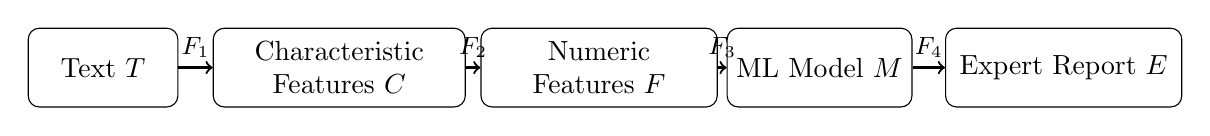
\begin{tikzpicture}[scale=1.0]
  % nodes (absolute positions to avoid the positioning library)
  \node[draw,rounded corners,align=center,minimum width=1.9cm,minimum height=1.0cm] at (0,0) (t) {Text $T$};
  \node[draw,rounded corners,align=center,minimum width=3.2cm,minimum height=1.0cm] at (3.0,0) (c) {Characteristic\\Features $C$};
  \node[draw,rounded corners,align=center,minimum width=3.0cm,minimum height=1.0cm] at (6.3,0) (f) {Numeric\\Features $F$};
  \node[draw,rounded corners,align=center,minimum width=2.3cm,minimum height=1.0cm] at (9.1,0) (m) {ML Model $M$};
  \node[draw,rounded corners,align=center,minimum width=3.0cm,minimum height=1.0cm] at (12.2,0) (e) {Expert Report $E$};
  \draw[->,thick] (t) -- node[above]{\small $F_1$} (c);
  \draw[->,thick] (c) -- node[above]{\small $F_2$} (f);
  \draw[->,thick] (f) -- node[above]{\small $F_3$} (m);
  \draw[->,thick] (m) -- node[above]{\small $F_4$} (e);
\end{tikzpicture}
\caption{End-to-end mental-model approximation pipeline.\label{fig:pipeline}}
\end{figure}

%%%%%%%%%%%%%%%%%%%%%%%%%%%%%%%%%%%%%%%%%%
\section{Discussion}

\subsection{Comparison with Prior Studies}
Relative to classical ML, our approach retains interpretability but avoids brittle, vocabulary-bound representations by combining LLM-guided discovery with deterministic computation. Compared with deep BERT-based detectors \cite{kaliyar2021fakebert,keya2021augfakebert}, the proposed proxy focuses on traceability: each numeric feature is linked to concrete evidence (tokens, quotes, external checks), enabling expert auditing that model-agnostic post-hoc tools (e.g., LIME/Anchors) approximate from the outside \cite{lime,anchors}.

\subsection{Advantages and Disadvantages}

Advantages.

(i) Explicit feature definitions and metadata promote reproducibility and explainability. (ii) Human-in-the-loop visualization (PCA/MDS/t-SNE) helps detect leakage and dataset biases early. (iii) The expert report template translates model decisions into audit-ready evidence.

Disadvantages.

(i) Feature engineering requires careful maintenance as misinformation tactics evolve. (ii) LLM-assisted $F_1$ may introduce prompt sensitivity; we mitigate this with deterministic $F_2$. (iii) Reported in-domain baselines are high; generalization must be verified with out-of-distribution tests and source de-duplication \cite{amer2021context,villela2023review}.

\subsection{Limitations and Open Questions}
The PDFs provide partial numeric results for SVM experiments; thus we refrain from reporting specific values not present in the sources. Open questions include: faithfulness measurement between the proxy and an underlying LLM; robustness to LLM style attacks \cite{wu2023sheep,park2024adstyle}; and detection bias against LLM-generated text \cite{su2023biased}. Extending the feature set to multimodal signals (images, video) along the lines of LVLM-based detectors is a priority \cite{liu2024fkaowl}.

%%%%%%%%%%%%%%%%%%%%%%%%%%%%%%%%%%%%%%%%%%
\section{Conclusions}

This study presented a principled pipeline for explainable fake news detection that approximates the decisions of large language models within a compact, auditable mental model. The method is grounded in four formal mappings (from text to characteristic features, to numeric features, to a transparent ML proxy, and finally to an expert report) that collectively enforce traceability from the final decision back to concrete evidence in the text. An explicit library of feature mechanisms operationalizes domain knowledge into $[0,1]$-valued quantities and retains the spans, quotes, and external references that influenced each value, enabling faithful post-processing such as token-level annotation. A rigorous evaluation protocol was specified: stratified train--test splits, visual analytics using PCA/MDS/t-SNE to confirm separability and detect leakage, and standard metrics (accuracy, precision, recall, F1, and AUC) to summarize classification quality. We also included a comparison with reported baselines in the literature to situate the proxy’s expected performance relative to deep learning methods. Beyond detection accuracy, the central outcome is improved accountability: the generated expert report links each decision to interpretable features and human-understandable rationales, thereby supporting auditing, error analysis, and trustworthy deployment in settings where the cost of misclassification is high.

The primary limitations of the current work are practical rather than conceptual. First, the provided PDFs contain partial numerical results for SVM training; therefore, we intentionally abstained from reproducing absent values. Second, prompt sensitivity at the feature-discovery stage can introduce stochastic variation; our design mitigates this through deterministic numeric computation and metadata capture but cannot eliminate it entirely. Third, like most text-only systems, the pipeline does not yet leverage images or video that often accompany news items.

Future research will focus on three directions: (i) measuring and improving faithfulness between the proxy and an underlying LLM with causal and counterfactual tests; (ii) enhancing robustness against adversarial style attacks and distribution shifts via augmentation and continual learning; and (iii) extending the feature set to multimodal evidence and external knowledge integration to elevate both accuracy and explanatory depth. Taken together, the proposed framework offers a practical path to reconcile the high competence of LLMs with the transparency requirements of explainable AI, yielding decisions that are not only competitive but also inspectable and defensible.

%%%%%%%%%%%%%%%%%%%%%%%%%%%%%%%%%%%%%%%%%%
\authorcontributions{Conceptualization, P.R. and O.B.; methodology, P.R.; software, P.R.; validation, P.R., O.B. and I.K.; formal analysis, P.R. and I.K.; investigation, P.R.; resources, O.B.; data curation, P.R.; writing---original draft preparation, P.R.; writing---review and editing, P.R., O.B. and I.K.; visualization, P.R.; supervision, I.K.; project administration, O.B. All authors have read and agreed to the published version of the manuscript.}

\funding{This research received no external funding.}

\institutionalreview{Not applicable.}

\informedconsent{Not applicable.}

\dataavailability{No new data were created in this study. Replication requires publicly available datasets (e.g., ISOT and LIAR) and the feature mechanisms described herein.}

\acknowledgments{We thank the maintainers of open-source NLP libraries used in prototyping.}

\conflictsofinterest{The authors declare no conflicts of interest. The funders had no role in the design of the study; in the collection, analyses, or interpretation of data; in the writing of the manuscript; or in the decision to publish the results.}

\abbreviations{Abbreviations}{
\begin{tabular}{@{}ll}
LLM & Large Language Model\\
xAI & Explainable Artificial Intelligence\\
MDS & Multidimensional Scaling\\
PCA & Principal Component Analysis\\
t-SNE & t-Distributed Stochastic Neighbor Embedding\\
SVM & Support Vector Machine\\
AUC & Area Under the Curve\\
\end{tabular}
}

%%%%%%%%%%%%%%%%%%%%%%%%%%%%%%%%%%%%%%%%%%
\appendixtitles{yes}
\appendixstart
\appendix

\section{Formalizing the Approximation}\label{sec:appendixA}

Let us consider a standard supervised learning task, such as fake news detection, with a labeled training dataset. Our goal is to explain the decisions of a powerful but opaque DL model (specifically, an LLM) using a simpler, more interpretable ML model.

We begin by representing the data through two different ``lenses.'' First, we process the training dataset (composed of $m$ text samples) through the LLM to obtain a set of high-dimensional embedding vectors. These embeddings capture the rich semantic content of the text as understood by the LLM. We represent these embeddings as a matrix $A$ of size $m \times k$, where $m$ is the number of samples and $k$ is the dimensionality of the LLM embeddings. Each row of $A$ corresponds to a text sample, and each column represents a dimension in the LLM's latent feature space.
\begin{equation}
A = \begin{pmatrix}
 a_1^1 & a_1^2 & \dots & a_1^k \\
 a_2^1 & a_2^2 & \dots & a_2^k \\
 \vdots & \vdots & \ddots & \vdots \\
 a_m^1 & a_m^2 & \dots & a_m^k 
\end{pmatrix}.
\end{equation}

Second, for the same $m$ text samples, we derive a corresponding set of features based on a ``mental model''---a set of characteristics that a human expert would use to judge the content. For fake news, these could be features like ``degree of emotional language,'' ``subjectivity score,'' ``presence of sensationalism,'' etc. We represent these expert-defined features as a matrix $B$ of size $m \times l$, where $l$ is the number of interpretable features. Typically, $l$ is much smaller than $k$.
\begin{equation}
B = \begin{pmatrix}
 b_1^1 & b_1^2 & \dots & b_1^l \\
 b_2^1 & b_2^2 & \dots & b_2^l \\
 \vdots & \vdots & \ddots & \vdots \\
 b_m^1 & b_m^2 & \dots & b_m^l 
\end{pmatrix}.
\end{equation}

The central problem is to find a transformation that maps the opaque LLM representations in $A$ to the interpretable representations in $B$. We seek a transition matrix $T$ of size $k \times l$ that can achieve this mapping. In an ideal scenario, we would have a direct linear relationship:
\begin{equation}
B = A T.
\end{equation}

However, in practice, a perfect linear mapping is unlikely to exist, especially since the number of samples $m$ may not be equal to the feature dimensions $k$ or $l$, and the relationship between the feature spaces is more complex. Therefore, we aim to find a matrix $T$ that provides the best possible approximation in a least-squares sense. We want to find $T$ such that the Euclidean norm of the difference between $A T$ and $B$ is minimized:
\begin{equation}
AT \approx B
\end{equation}

This is a classic problem in linear algebra, which can be solved using the pseudoinverse of matrix $A$. The Moore-Penrose pseudoinverse, denoted as $A^+$, provides the best least-squares solution for an overdetermined or underdetermined system of linear equations. The optimal transition matrix $T$ can thus be approximated as:
\begin{equation}
T \approx A^+ B.
\end{equation}

We compute the pseudoinverse $A^+$ using Singular Value Decomposition (SVD), which is a robust and standard method. Any matrix $A$ can be factorized as $A = U\Sigma V^T$, where $U$ and $V$ are orthogonal matrices and $\Sigma$ is a diagonal matrix containing the singular values of $A$. The pseudoinverse $A^+$ is then given by:
\begin{equation}
A^+ = V\Sigma^+U^T,
\end{equation}
where $\Sigma^+$ is formed by taking the reciprocal of each non-zero singular value in $\Sigma$ and then transposing the resulting matrix.

This method provides a stable way to compute the transition matrix $T$.

Once $T$ is computed, it encapsulates the learned relationship between the LLM's internal world and the human's mental model. For any new text sample, we can generate its LLM embedding, let's call it $a^*$ (a vector of size $1 \times k$). We can then use our transition matrix $T$ to project this embedding into the interpretable feature space and obtain the corresponding mental model vector, $b^*$ (a vector of size $1 \times l$):
\begin{equation}
b^* = a^* T.
\end{equation}

The elements of the resulting vector $b^*$ are the predicted values for our human-understandable features. For example, $b^*$ might tell us that the new text has a high score for ``sensationalism'' and a low score for ``factual confirmation,'' thereby providing a transparent and interpretable basis for classifying it as fake news.

%%%%%%%%%%%%%%%%%%%%%%%%%%%%%%%%%%%%%%%%%%

%===================== REFERENCES =======================

\reftitle{References}

\begin{adjustwidth}{-\extralength}{0cm}

\bibliography{references}

\PublishersNote{}

\end{adjustwidth}

\end{document}